\section{Analysis and results}
\label{sec:results}

\begin{table*}[t]
    \centering
    \begin{threeparttable}
    \begin{tabular}{||l|c|c|r||}
        \toprule
            Node type & Complexity & Memory cost & Communication cost \\
        \midrule \midrule
		    Prover & $O(n^2log(n))$ & $160+10*c$ & \vtop{\hbox{\strut (send) $64 + 96 * h$ }\hbox{\strut (recv) $32*g + 94$ }} \\
		\midrule
		    Aggregator & $O(n log(n))$ & $276+10*c+96*z$ & \vtop{\hbox{\strut (send) $(32*c+94)*nb + 64 + 96*z$}\hbox{\strut (recv) $(32*c+94) + 96* nb + 96*z$}} \\
		\midrule
		    Verifier & $O(n^2log(n))$ & - & - \\
		\midrule
	\end{tabular}
	\begin{tablenotes}
	    \item[1] n = number of bits in input
	    \item[2] z = number of bad neighbours
		  \item[3] c = number of counters
		  \item[4] h = 1 if bad prover, 0 otherwise
		  \item[5] g = number of good configurations  
    \end{tablenotes}
    \caption{Complexity, Memory and Communication costs for each node}
    \label{tab:1}
    \end{threeparttable}
\end{table*}


\subsection{Computational cost}
We now proceed to evaluate the computational, memory and communication costs of this works's SANA implementation for Provers and Aggregators.
Starting from the computational cost, the most complex functions of the protocol are the sign and verify functions as they both have
to perform operations on the elliptic curve. This operations require several multiplication to be executed.
Table~\ref{tab:1} report the estimations of the computational costs for the functions and the nodes using them. 
The variable \textbf{n} is the number of bits of the input given to the function, in this case n = 256 bits.\\
It can safely be said that the highest cost falls on the Provers while the Aggregators, which only have to perform one multiplication between objects, face lower computational load.
Memory costs for the Prover are contained as long as we choose a fair amount of counters. 
While for the aggregator are linearly dependet on the number of bad neighbours, as the node has to memorize the public key and the message of each compromised node.\\

For what concerns the theoretical communication costs of the protocol, 
the aggregator has to send and receive more bytes depending on how many compromised devices 
it has as its neighbours.\\

After dealing with the theoretical costs it's crucial to shift to the practical test in order to estimate the true work load for the nodes.
We ran several simulation to investigate the time required to perform each action of the protocol (signature, aggregation, verify...) and have a proper estimation of the total time of execution of the algorithm.
For this calculation we used this formula:
\[(\sum_{i=0}^{n} p_i) * t_{agg} + d * (t_{ver} + t_{hash}) + t_{sign} \]
Where \textbf{n} is the number of the provers and \textbf{d} is the depth of the tree generated from the algorithm.
This provides a lower bound for the execution time of the whole protocol as it relies on the fact that all node 
can sign simultaneously and that at each level of the tree all the challenge verifications from the aggregators require the same time.
Unfortunately this formula is not easy to use in real context as the devices move in space and the number of neighbours may change depending on the proximity of the other devices, so it's hard to assume what the depth of the tree can be and how much parallelization can happen while descending the tree.\\

Doing a comparison with the SANA's claims we obtained an higher comunication cost due to our keys being 512 bits long instead of 256 and the software configuration of provers being hashed to 256 bits.\\
Instead, memory costs for provers are lower in our implementation and in SANA's paper memory cost for the Aggregator are missing, so it's not possible to make a comparison.\\
Run-time costs are similar without considering the comunication time not present in our simulation.

\subsection{Aggregation cost}
For what concerns the duration of the process of aggregation the observation focussed on one Aggregator aggregating the signature of up to 1000 provers .
Firstly, the aggregation time increase linearly with the number of Provers connected to the same Aggregator.
But this same aggregation time is not suppose to scale with the number of compromised Provers.\\
Figure \ref{fig:aggregation_comparison} demonstrates the previuos claims by showing no relevant discrepancy beetween the 0\% 25\% 50\% 75\% and 100\% bad provers percentage.

\subsection{Verification cost}
The other parameter tested was the verification time of the Aggregator. 
The parameter were the number of provers and the percentage of them not signing the default message.\\
Theoretically the number of bad provers would make the verification time increase linearly, and on the other hand the verification time should be independent on the number of legitimate provers.
This is due to the fact that the legitimate Provers sign the default message, thus being verified in constant time.\\
Figure \ref{fig:verification_comparison} confirms that the time of verification is in fact independent from the number of provers if they are all legitimate (0\% bad provers).
Intsead, with 100\% of bad provers, the time for verification increase linearly with the number of provers, reaching up to 6000 seconds for the verification of 1000 bad provers.

\begin{figure}
  \centering
  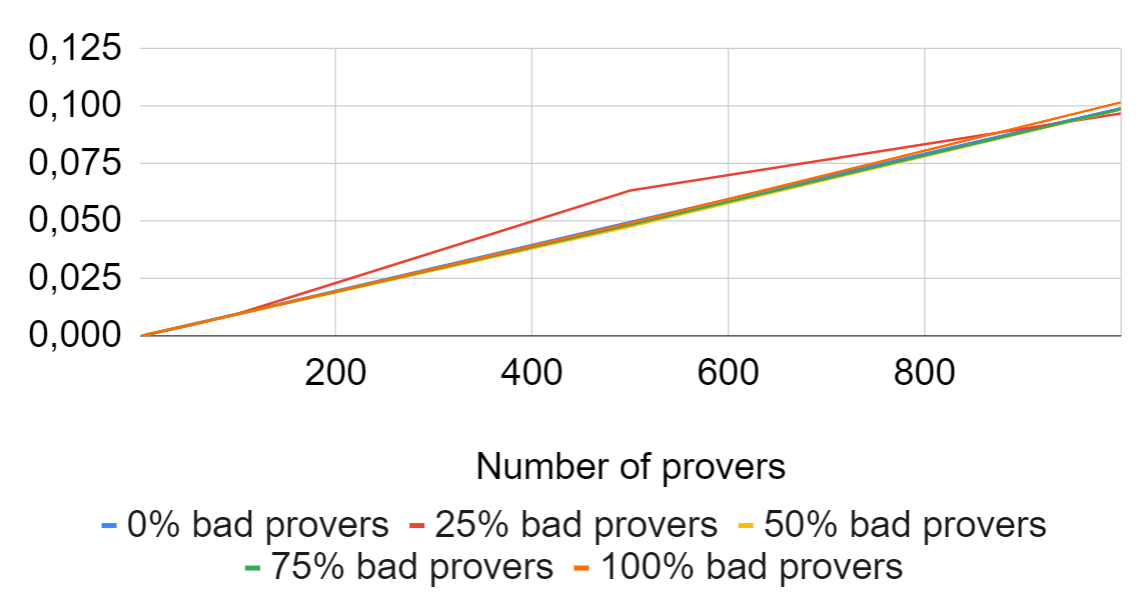
\includegraphics[width=.90\linewidth]{Images/aggregation.png}  
  \caption{Aggregation times comparison}
  \label{fig:aggregation_comparison}
\end{figure}
\begin{figure}
  \centering
  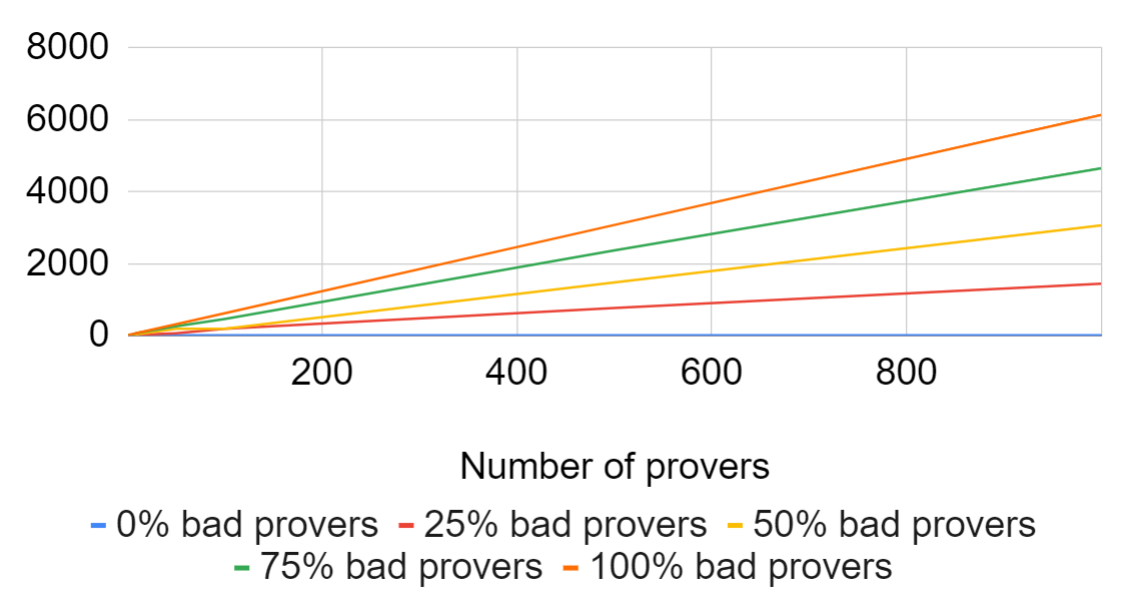
\includegraphics[width=.90\linewidth]{Images/verification.png}  
  \caption{Verification times comparison}
  \label{fig:verification_comparison}
\end{figure}
\begin{figure}
  \centering
	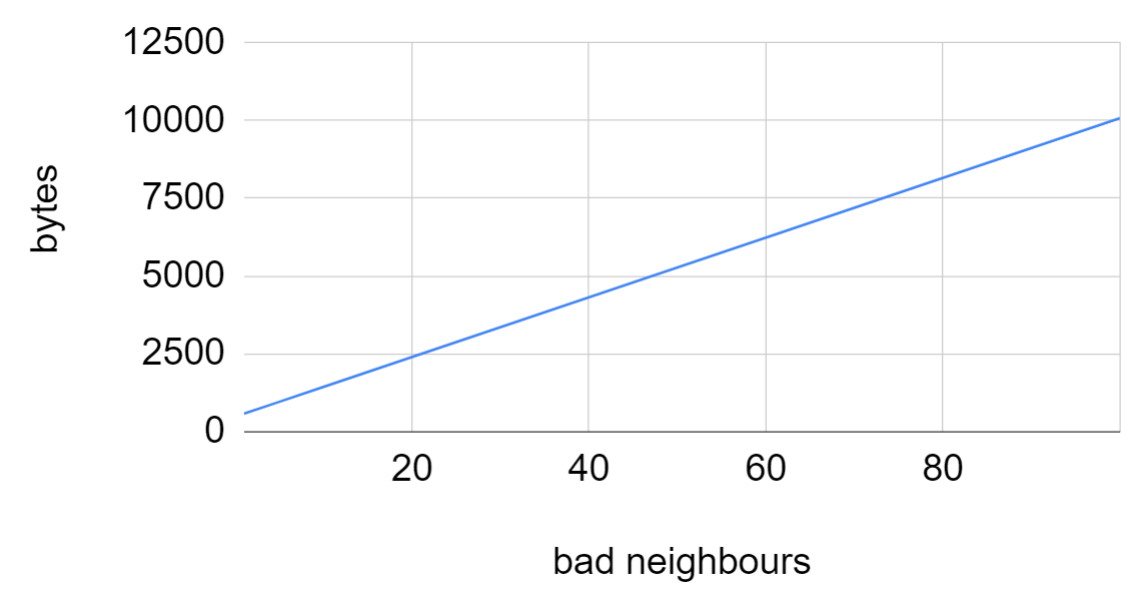
\includegraphics[width=.90\linewidth]{Images/memory_cost.png} 
	\caption{Memory cost for the aggregator} 
  \label{fig:memory_cost}
\end{figure}

\subsection{Memory cost}
In Figure \ref{fig:memory_cost} is represented the memory cost for the Aggregator.
Theoretically this is expected to increase linearly with the number of bad neighbours. This is due to the nature of the protocol identifying the compromised devices and storing public keys and message of all of them.\\
Figure \ref{fig:memory_cost} confirms this belief and shows how having more than just 19 bad provers make the Aggregator use more than 1024Kb of memory.\\


